\documentclass[a4paper,12pt]{article}
\usepackage[T1]{fontenc}
\usepackage{ninecolors}
\usepackage{booktabs}
\usepackage{caption}
\usepackage{tabularray}
\usepackage{hyperref}
\usepackage{graphicx}
\usepackage{subcaption}
\usepackage{parskip}
\usepackage{tikz}
\usepackage{circuitikz}
\usepackage{float}
\hypersetup{
  colorlinks=true,
  linkcolor=blue,
  filecolor=magenta,
  urlcolor=cyan,
  pdftitle={Lizard Kisses},
  pdfpagemode=FullScreen,
}
\graphicspath{ {img/} }
\captionsetup[table]{position=bottom}
\usepackage{geometry}
\usepackage{siunitx}
\usepackage{awesomebox}

\tikzset{
  padStyle/.style={line width=1mm, draw=orange, fill=none}
}

\tikzset{
  partStyle/.style={line width=1mm, draw=black, fill=none, rounded corners=4pt}
}

\begin{document}
\begin{titlepage}
  \vspace*{\stretch{1.0}}
  \begin{center}
    \Large\textbf{Lizard Kisses}\\
    \large{Overdrive pedal kit by Pedal Markt}
  \end{center}
  \vspace*{\fill}
  \begin{center}
    \today
  \end{center}
\end{titlepage}

\tableofcontents
\pagebreak

\section{Introduction}
Lizard Kisses is a color and texture device. With different
clipping and brightness options, it can act as a boost, an
overdrive, or a distortion. It stacks well with other pedals,
responds to your playing, and is a classy beast all around!

Lizard Kisses enclosure was designed by \href{https://fiz.gallery/}{Agata Fiz.}

\begin{figure}[h!]
  \centering
  \begin{subfigure}[b]{0.49\textwidth}
    \centering
    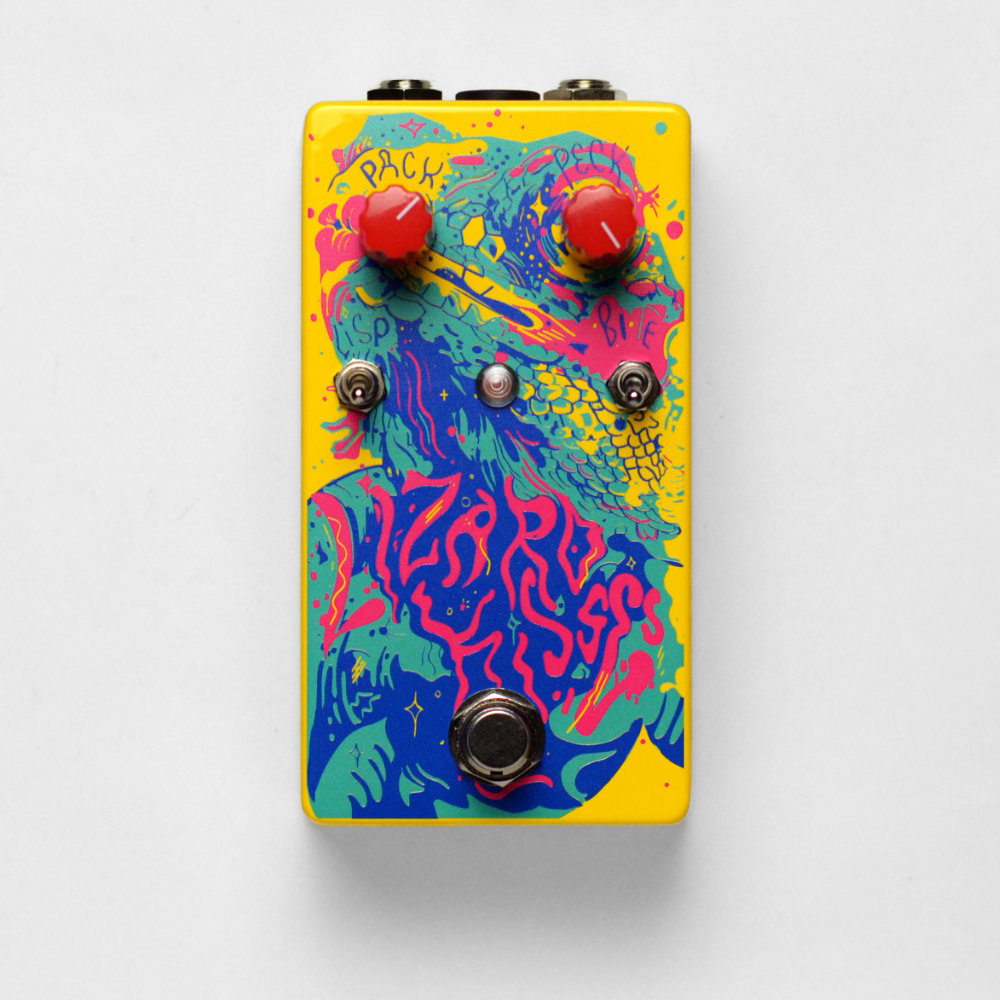
\includegraphics[width=\textwidth]{lizard-kisses-1000px.jpg}
  \end{subfigure}
  \begin{subfigure}[b]{0.49\textwidth}
    \centering
    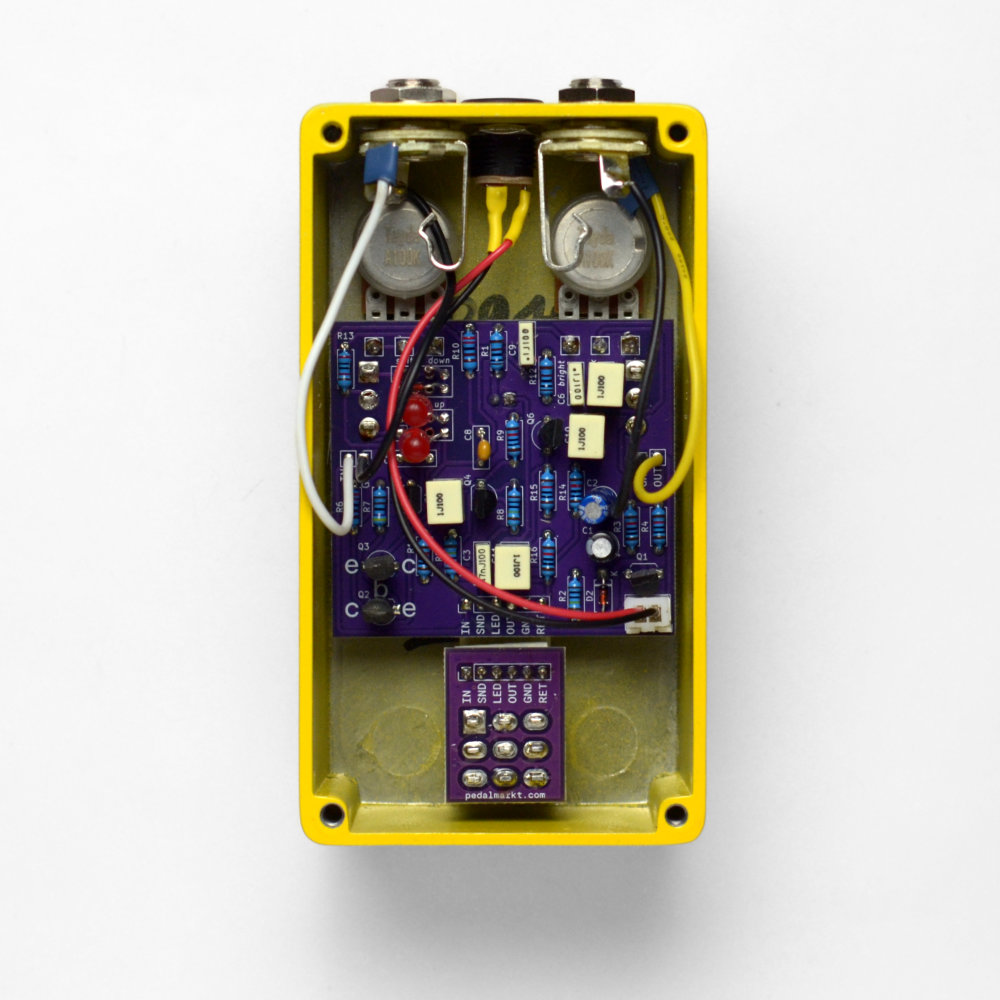
\includegraphics[width=\textwidth]{lizard-kisses-inside-1000px.jpg}
  \end{subfigure}
  \caption{Lizard Kisses: oustide and inside}
  \label{fig:lk}
\end{figure}

The pedal was originally conceived for the workshops at
\href{https://pedalmarkt.com}{Pedal Markt.} The intention
was  to make it as easy to build and customize as possible.

You will find the stock values for components in the
\hyperref[sec:bom]{BOM} below. There are separate sections
further in the document that describe how you could try out
alternative parts to get different sounds.

The circuit is based around a discrete operational
amplifier. Discrete means it's built out of single
transistors, as opposed to an integrated circuit aka a chip.
You can find \hyperref[sec:schematic]{the schematic} and
\hyperref[sec:circuit]{the circuit breakdown} further in the
document.

\pagebreak

\section{BOM – Bill of Materials}
\label{sec:bom}

BOM is a document that lists the parts you'd need to build a
project. Each row corresponds to a component with a certain
value, for example, a `ceramic capacitor with value 1nF.`
There could be one or more actual physical parts per
row, their designators are listed in the \textit{Reference}
column.

\tipbox{
  Components in the BOM are listed in order of assembly. Go
  through the table top to bottom. If you haven't built a
  kit before, check out the
  \hyperref[sec:steps]{Step-by-step Instructions} first.
}

\tipbox{
  In the BOM \textit{text in italic font} gives tips about how to mount or
  solder parts.
}

\tipbox{
  If you'd like to experiment with some of the parts, for
  example, \hyperref[sec:caps]{Brightness Caps} and
  \hyperref[sec:clip]{Clipping Diodes,} please socket them.
  Guides for that are in the respective sections.
}

\newgeometry{hmargin={1cm}}

\begin{longtblr}[caption = {BOM}]{
  hlines,
  vlines,
  rows={ht=1.2em},
  row{even}={bg=gray9},
  row{1}={bg=gray3,fg=white},
  width=\linewidth,
  colspec={lX[1]llX[2]},
}
  \hspace{1em}
  & \textbf{Ref}
  & \textbf{Value}
  & \textbf{Qnty}
  & \textbf{Description}
  \\
  \SetCell[c=5]{c,bg=gray6,fg=white}\textbf{Outboard}
  \\
  \hspace{1em}
  & -- & Enclosure & 1 & \textit{Mount both pots, both
  toggle switches, DC jack, Footswitch and LED Lampshade
  into the enclosure before soldering}
  \\
  \hspace{1em}
  & -- & Lampshade & 1
  & Small transparent plastic part for the LED,
  \textit{mount in enclosure before putting the boards in}
  \\
  \hspace{1em}
  & -- & Rubber Ring & 1
  & \textit{Use it to keep LED Lampshade in place}
  \\
  \hspace{1em}
  & -- & DC Jack & 1
  & Black plastic part with a nut, \textit{mount in
  enclosure before soldering}
  \\
  \hspace{1em}
  & -- & DC Cable & 1
  & Red and black cables in a JST connector, \textit{cut to
  $\approx12cm$ and solder to DC Jack once it's mounted in enclosure}
  \\
  \hspace{1em}
  & -- & Audio Jack & 2 & \textit{Only mount these in the
  enclosure together with the main board once they are wired up}
  \\
  \SetCell[c=5]{c,bg=gray6,fg=white}\textbf{Main board, floor side}
  \\
  \hspace{1em}
  & GND & Wire & 2 & $\approx10cm$, black, \textit{strip and
  tin the ends}
  \\
  \hspace{1em}
  & IN & Wire & 1 & $\approx10cm$, any color, \textit{strip and tin
  the ends}
  \\
  \hspace{1em}
  & OUT & Wire & 1 & $\approx10cm$, any other color,
  \textit{strip and tin the ends}
  \\
  \hspace{1em}
  & R7 & 4.7k & 1 & Resistor
  \\
  \hspace{1em}
  & R13 & 20k & 1
  & Resistor
  \\
  \hspace{1em}
  & R1 & 1k & 1
  & Resistor for the LED, \textit{larger value will make the LED
  dimmer, values up to 6.8k are reasonable}
  \\
  \hspace{1em}
  & R12 & 1k & 1
  & Resistor
  \\
  \hspace{1em}
  & R6, R10 & 2.2k & 2
  & Resistor
  \\
  \hspace{1em}
  & R2, R5, R8 & 1M & 3
  & Resistor
  \\
  \hspace{1em}
  & R3, R4, R9, R11, R14, R15, R16 & 10k & 7
  & Resistor
  \\
  \hspace{1em}
  & D2 & 1N4148 & 1
  & Diode, \textit{orientation matters}
  \\
  \hspace{1em}
  & switch up & 1N4148 & 3
  & See \hyperref[sec:clip]{Clipping Diodes} section
  \\
  \hspace{1em}
  & Q1 & TP0606 & 1
  & P-channel MOSFET, \textit{orientation matters}
  \\
  \hspace{1em}
  & Q5 & 2N3906 & 1
  & PNP transistor, \textit{orientation matters}
  \\
  \hspace{1em}
  & Q2, Q3, Q4, Q6 & 2N3904 & 4
  & NPN transistor, \textit{orientation matters}
  \\
  \hspace{1em}
  & C5, C8 & 47p & 2
  & Ceramic capacitor
  \\
  \hspace{1em}
  & C3 & 47n & 1
  & Film capacitor
  \\
  \hspace{1em}
  & C9 & 100n & 1
  & Film capacitor
  \\
  \hspace{1em}
  & C6 (bright) & 330n & 1
  & See \hyperref[sec:caps]{Brightness capacitors} section
  \\
  \hspace{1em}
  & C7 (dark) & 470n & 1
  & See \hyperref[sec:caps]{Brightness capacitors} section
  \\
  \hspace{1em}
  & -- & Power Socket & 1
  & 2-pin JST on the bottom-left of the board,
  \textit{orientation matters}
  \\
  \hspace{1em}
  & switch down & Red LED & 2
  & See \hyperref[sec:clip]{Clipping Diodes} section
  \\
  \hspace{1em}
  & C4, C10, C11 & 1u & 3
  & Film capacitor
  \\
  \hspace{1em}
  & C1 & 100u & 1
  & Electrolytic capacitor, \textit{orientation matters}
  \\
  \hspace{1em}
  & C2 & 47u & 1
  & Electrolytic capacitor, \textit{orientation matters}
  \\
  \SetCell[c=5]{c,bg=gray6,fg=white}\textbf{Main board, player side}
  \\
  \hspace{1em}
  & -- & Ribbon cable & 1
  & Pads for that cable are in the bottom-center of the main
  board, \textit{solder one end to main board, another to
  switch board, \textbf{make sure pin names on the two
  boards match, IN on one board is connected to IN on the
  other board etc}} \\
  \hspace{1em}
  & VOL, GAIN  & A100k & 2
  & Potentiometers, \textit{mount in enclosure before
  soldering}
  \\
  \hspace{1em}
  & BRIGHT & On-On & 1
  & 2-position switch, \textit{mount in enclosure before soldering}
  \\
  \hspace{1em}
  & CLIP & On-Off-On & 1
  & 3-position switch, \textit{mount in enclosure before soldering}
  \\
  \hspace{1em}
  & -- & LED & 1
  & \textit{Insert in PCB first. Solder last, once the
  main board is in the enclosure. Orientation matters}
  \\
  \SetCell[c=5]{c,bg=gray6,fg=white}\textbf{Switch board, player side}
  \\
  \hspace{1em}
  & -- & Footswitch & 1
  & Switch, \textit{mount in enclosure before putting the boards in}
  \\
\end{longtblr}
\label{tbl:BOM}

\restoregeometry{}

\subsection{Note on values}

Different kits and schematics designate values differently.
For example, these usually mean the same value:
\\
$\SI{2.2}{\kohm} = 2.2k = 2k2 = 2.2 \times 10^{3} Ohm = 2200Ohm$
\\
$\SI{4.7}{\uF} = 4.7u = 4u7 = 4.7 \times 10^{-6} Farad = 0.0000047 Farad$

\begin{table}[h!]
  \caption{Component values}
  \centerline{
    \begin{tblr}{
      hlines,
      vlines,
      rows={ht=1.2em},
      row{1}={bg=gray3,fg=white},
      colspec={Xrr}
    }
      \textbf{Value}
      & \textbf{Multiplier}
      & \textbf{Unit}
      \\
      \SetCell[c=3]{c}\textbf{Resistance}
      \\
      \SI{100}{\ohm}, 100R, 100 & 1 & Ohm
      \\
      \SI{1}{\kohm}, 1k & $10^{3}$ & Ohm
      \\
      \SI{1}{\Mohm}, 1M & $10^{6}$ & Ohm
      \\
      \SetCell[c=3]{c}\textbf{Capacitance}
      \\
      \SI{1}{\pF}, 1p & $10^{-12}$ & Farad
      \\
      \SI{1}{\nF}, 1n & $10^{-9}$ & Farad
      \\
      \SI{1}{\uF}, 1u & $10^{-6}$ & Farad
    \end{tblr}
  }
\end{table}

\pagebreak

\section{Clipping Diodes}
\label{sec:clip}

There could be two sets of clipping diodes in Lizard
Kisses. The on-off-on 'BITE' switch toggles between one of
the two sets (on) or no diodes in the middle (off) position.

There are 8 pads per each (on) position of the switch you can
use to insert diodes. Pads 2 and 3, 6 and 7 are connected by
the PCB.

\begin{figure}[h!]
\centering
\begin{tikzpicture}
%\draw[help lines] grid(10,4);

\foreach \c in {1}
{
  \draw[padStyle] (4+0.2,\c) -- (6-0.2,\c);
  \draw[padStyle] (4+0.2,\c+2) -- (6-0.2,\c+2);

  \foreach \x [count=\xi] in {2,4,6,8}
  {
    \foreach \y [count=\yi] in {0,2}
    {
      \filldraw[padStyle] (\x, \c + \y) circle (0.2);
      \pgfmathsetmacro\pin{int(add(\xi,multiply(4,add(-1,\yi)))};
      \node at (\x, \c + \y - 0.5) {\pin};
    }
  }
}

\end{tikzpicture}
\caption{Pads for a single set of diodes}
\end{figure}


\pagebreak

\subsection{Stock clipping setup}

The stock clipping diode combinations are:

\begin{itemize}
  \item \textbf{switch down:} two red LEDs, pointing in
    opposite directions. That combo leads to symmetrical
    clipping around \SI{1.6}{\V}.
  \item \textbf{switch up:} two 1N4148 silicon diodes in
    series, pointing in one direction, one 1N4148 pointing
    in the other direction. That combo leads to asymmetrical
    clipping. One part of the waveform will be clipped
    around \SI{0.7}{\V}, another around \SI{1.4}{\V}
\end{itemize}

\begin{figure}[h!]
\centering
\begin{tikzpicture}
  % \draw[help lines] grid(10,14);
  \node at (5,13.5) {\large switch down};
  \node at (5,5.5) {\large switch up};

  \foreach \c in {1,9}
  {
    \draw[padStyle] (4+0.2,\c) -- (6-0.2,\c);
    \draw[padStyle] (4+0.2,\c+2) -- (6-0.2,\c+2);
    \draw[dashed,gray] (0,\c-1) -- (10,\c-1) -- ++(0,6) -- ++(-10,0) -- cycle;
    \foreach \x [count=\xi] in {2,4,6,8}
    {
      \foreach \y [count=\yi] in {0,2}
      {
        \filldraw[padStyle] (\x, \c + \y) circle (0.2);
        \pgfmathsetmacro\pin{int(add(\xi,multiply(4,add(-1,\yi)))};
        \node at (\x, \c + \y - 0.5) {\pin};
      }
    }
  }

  \draw[partStyle]
    (2,1)
    -- ++(0,1)
    -- (4.5,2)
    +(0, 0.5)
    -- +(0, -0.5)
    ++(0,0)
    -- +(1,0.5)
    -- +(1,-0.5)
    -- +(0,0)
    ++(1,0)
    -- (8,2)
    -- ++(0,-1);

  \draw[partStyle]
    (2,3)
    -- ++(0,1)
    -- ++(0.5,0)
    +(0, 0.5)
    -- +(0, -0.5)
    -- +(1,0)
    -- +(0,+0.5)
    ++(1,0)
    +(0,0.5)
    -- +(0,-0.5)
    ++(0,0)
    -- ++(0.5,0)
    -- +(0,-1);

  \draw[partStyle]
    (6,3)
    -- ++(0,1)
    -- ++(0.5,0)
    +(0, 0.5)
    -- +(0, -0.5)
    -- +(1,0)
    -- +(0,+0.5)
    ++(1,0)
    +(0,0.5)
    -- +(0,-0.5)
    ++(0,0)
    -- ++(0.5,0)
    -- +(0,-1);

  \draw[partStyle]
    (2,9)
    -- ++(0,1)
    -- ++(2.5,0)
    +(0, 0.5)
    -- +(0, -0.5)
    ++(0,0)
    -- +(1,0.5)
    -- +(1,-0.5)
    -- +(0,0)
    ++(1,0)
    -- ++(2.5,0)
    -- ++(0,-1);

  \draw[partStyle]
    (2,11)
    -- ++(0,1)
    -- ++(2.5,0)
    +(0, 0.5)
    -- +(0, -0.5)
    -- +(1,0)
    -- +(0,+0.5)
    ++(1,0)
    +(0,0.5)
    -- +(0,-0.5)
    ++(0,0)
    -- ++(2.5,0)
    -- +(0,-1);

\end{tikzpicture}
\caption{Stock clipping setup}
\end{figure}

\subsection{Experiments with diodes}

If you'd like to play with different
combinations of diodes, I'd recommend putting four 4-pin
sockets into each row of pads. Two 4-pin sockets for the
"switch up" position, two 4-pin sockets for the "switch
down" position.

For each of the two toggle positions you could try:

\begin{itemize}
  \item Mixing types of diodes, for example, silicon pointing
    in one direction, LED in the opposite direction;
  \item Putting diodes in series to increase the clipping
    voltage.
\end{itemize}

\tipbox{
  The higher the clipping voltage the less distorted the
  signal will be.
}

\tipbox{
Different types of diodes will lead to different clipping
  voltages. Roughly speaking here are some types of diodes in
  order of increasing clipping voltage: germanium diodes,
  silicon diodes, Red LEDs, Blue LEDs.
}

\tipbox{
  Putting diodes in series doubles the clipping
  voltage.
}

\pagebreak

\section{Brightness Capacitors}
\label{sec:caps}

The LISP switch on Lizard Kisses toggles between a single
bright capacitor, and bright+dark capacitors in parallel. By
putting capacitors in parallel, we add their values together
to get a darker sound. The way the circuit is set up, the
larger the value of overall capacitance, the more low-end
goes through.

The stock capacitor values are:

\begin{itemize}
  \item bright: \SI{330}{\nF}
  \item dark: \SI{470}{\nF}
\end{itemize}

If you'd like to experiment with putting other capacitor values,
socket the two capacitor slots. I'd recommend cutting short
the middle pin of a 3-pin socket.

As for the values to try, the lower the capacitor value the
less low-end will go through. The reasonable range of values
to try is between \SI{10}{\nF} and \SI{4.7}{\uF}.

\pagebreak

\section{Step-by-step Instructions}
\label{sec:steps}

\subsection{Mount parts on enclosure}

\begin{itemize}
  \item Mount the pots, the toggle switches, the lampshade,
    the DC jack, and the footswitch on the enclosure as
    shown below;
  \item Cut to $\approx12cm$ and pre-tin the ends of DC cables;
  \item Solder the DC cable to the DC jack.
\end{itemize}

\newgeometry{vmargin={3cm}, hmargin={1cm}}

\begin{figure}[h!]
  \centering
  \begin{subfigure}[b]{0.49\textwidth}
    \centering
    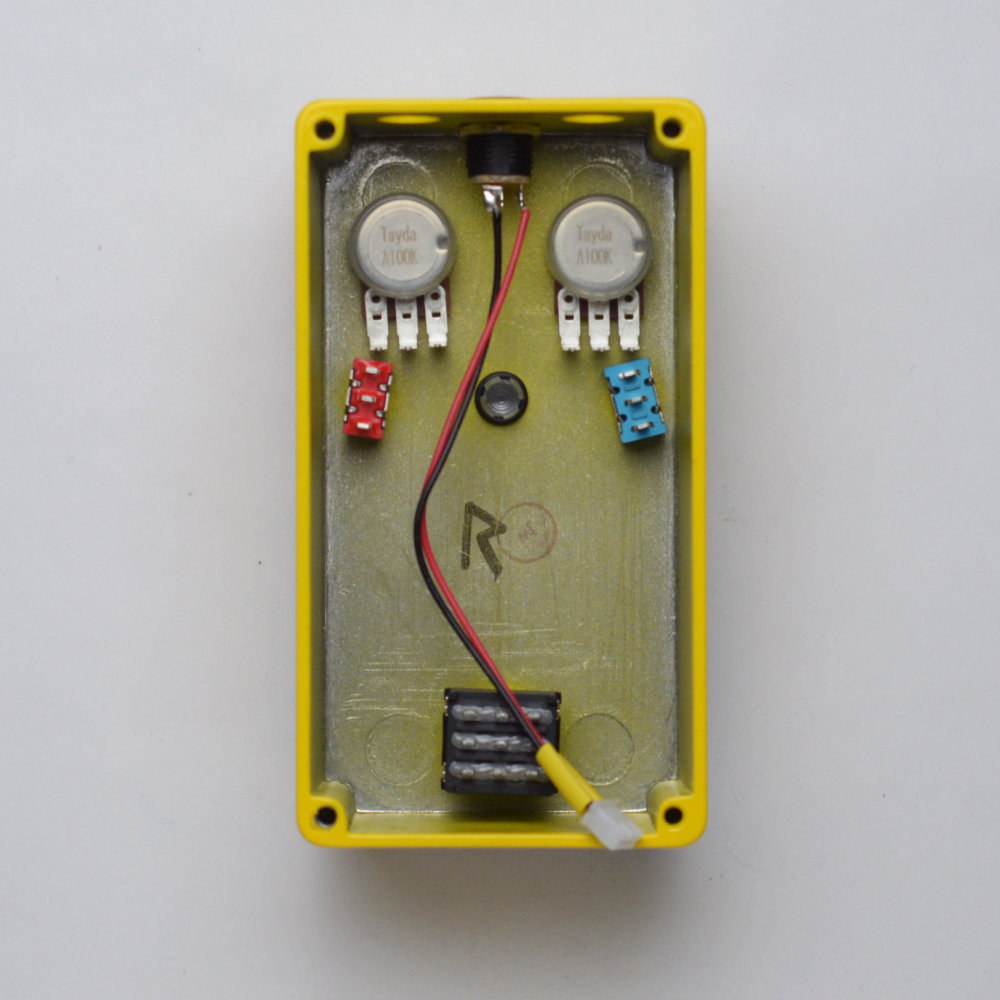
\includegraphics[width=\textwidth]{build/09-enclosure-mount-inside-1000px.jpg}
  \end{subfigure}
  \begin{subfigure}[b]{0.49\textwidth}
    \centering
    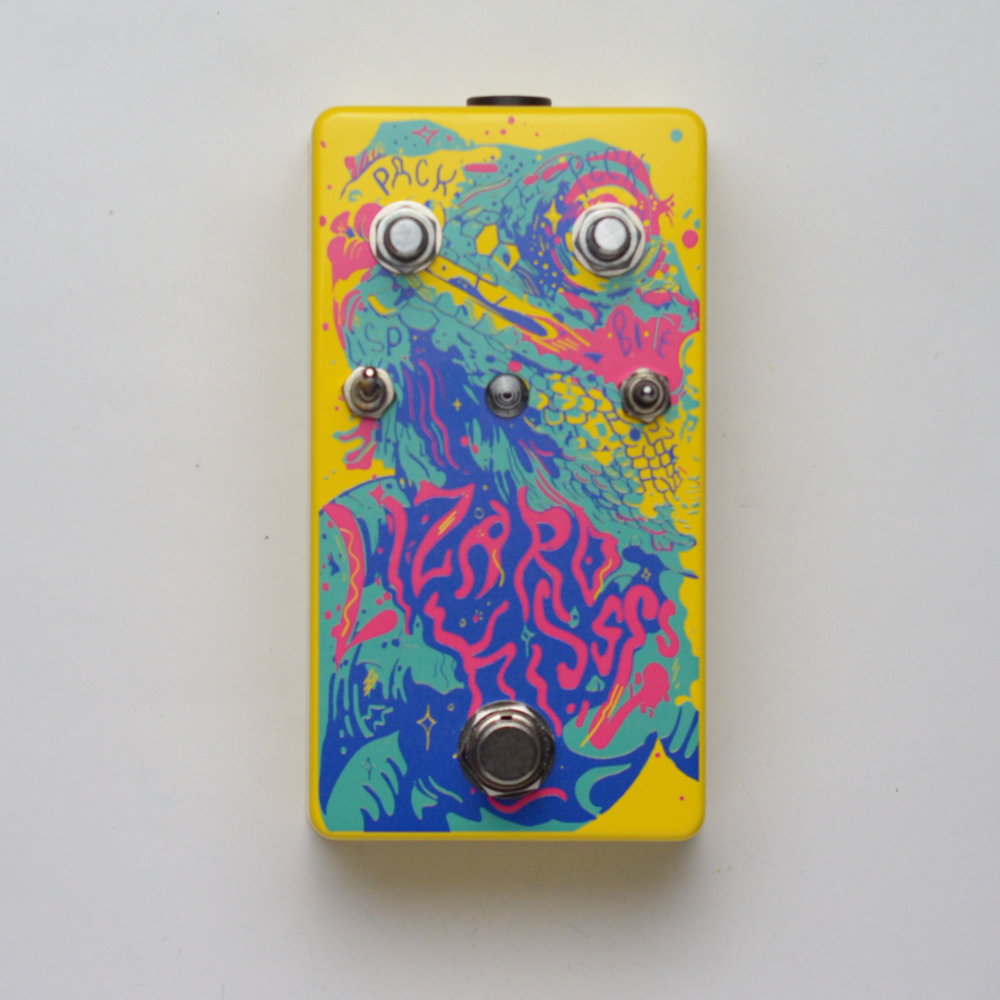
\includegraphics[width=\textwidth]{build/08-enclosure-mount-1000px.jpg}
  \end{subfigure}
  \caption{Inside and outside of the enclosure with parts
  mounted}
\end{figure}

\begin{figure}[h!]
  \centering
  \begin{subfigure}[b]{0.49\textwidth}
    \centering
    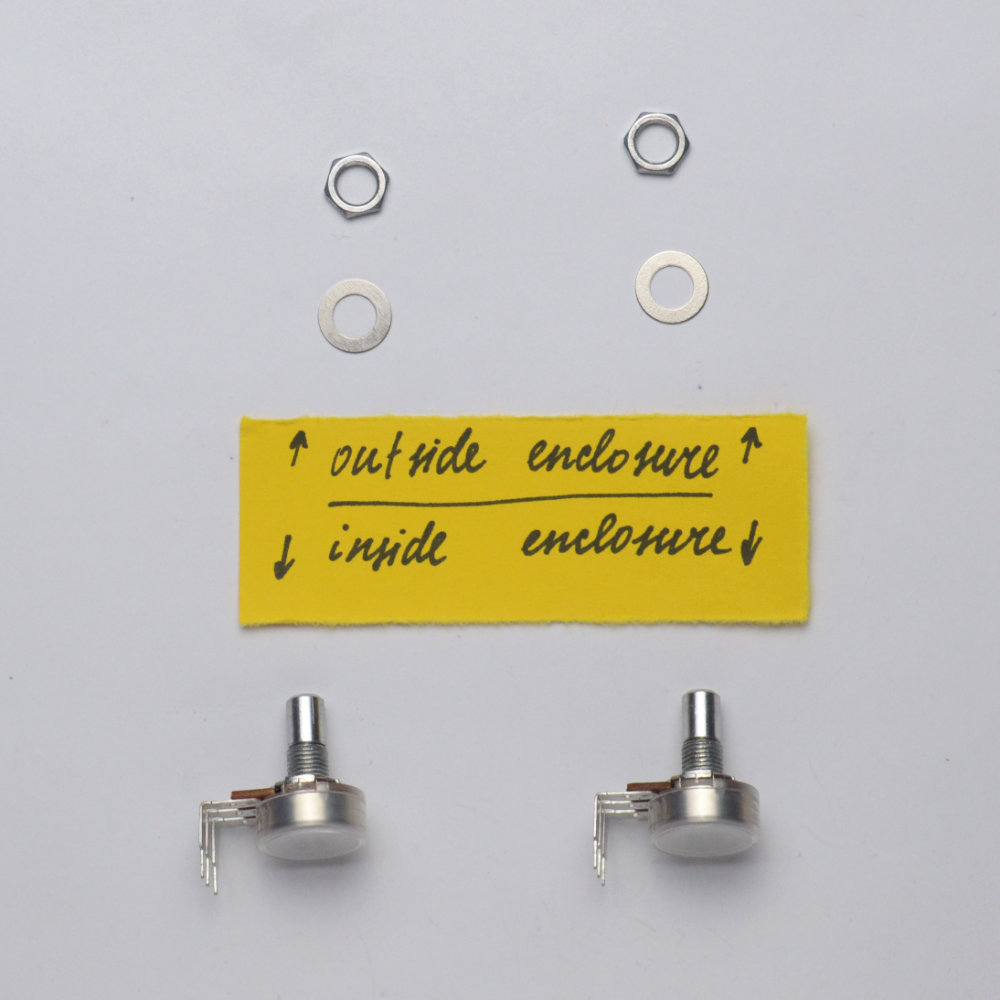
\includegraphics[width=\textwidth]{build/04-pots-mount-1000px.jpg}
  \end{subfigure}
  \begin{subfigure}[b]{0.49\textwidth}
    \centering
    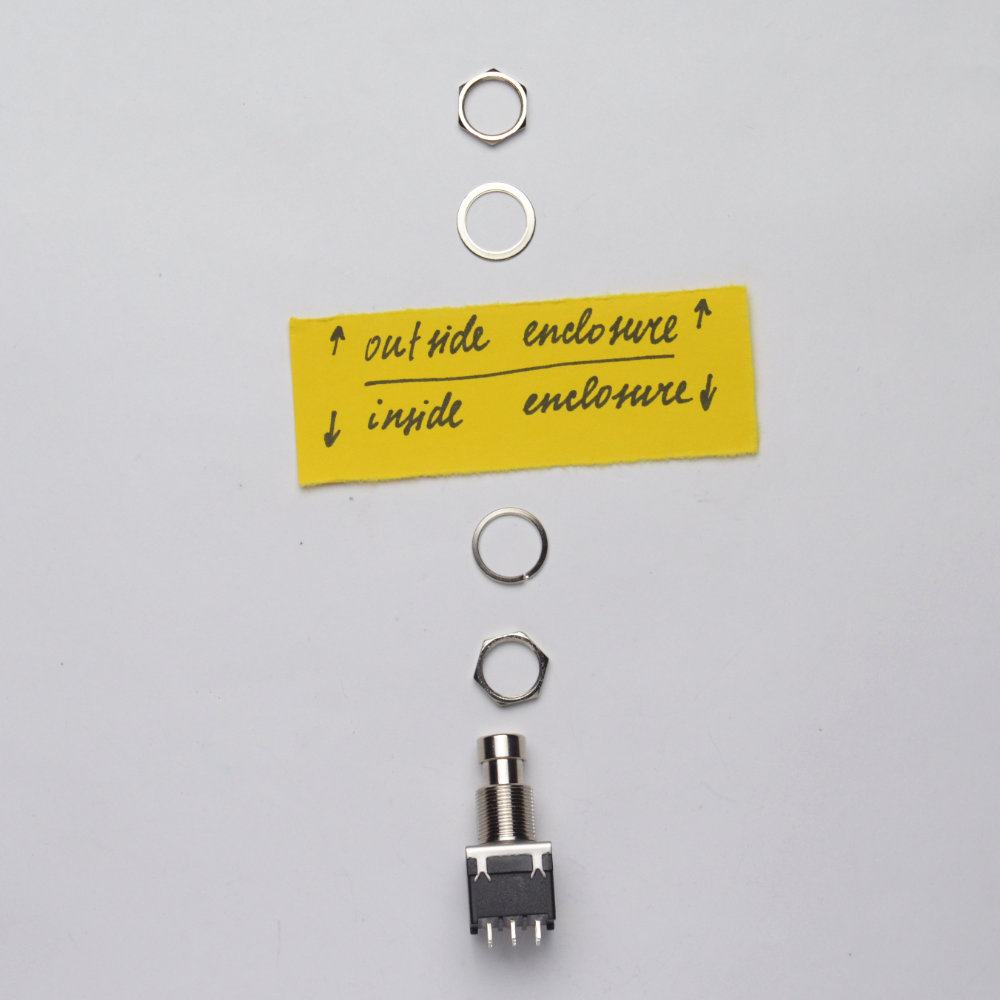
\includegraphics[width=\textwidth]{build/05-fs-mount-1000px.jpg}
  \end{subfigure}
  \caption{How to mount potentiometers and the footswitch}
\end{figure}

\begin{figure}[h!]
  \centering
  \begin{subfigure}[b]{0.49\textwidth}
    \centering
    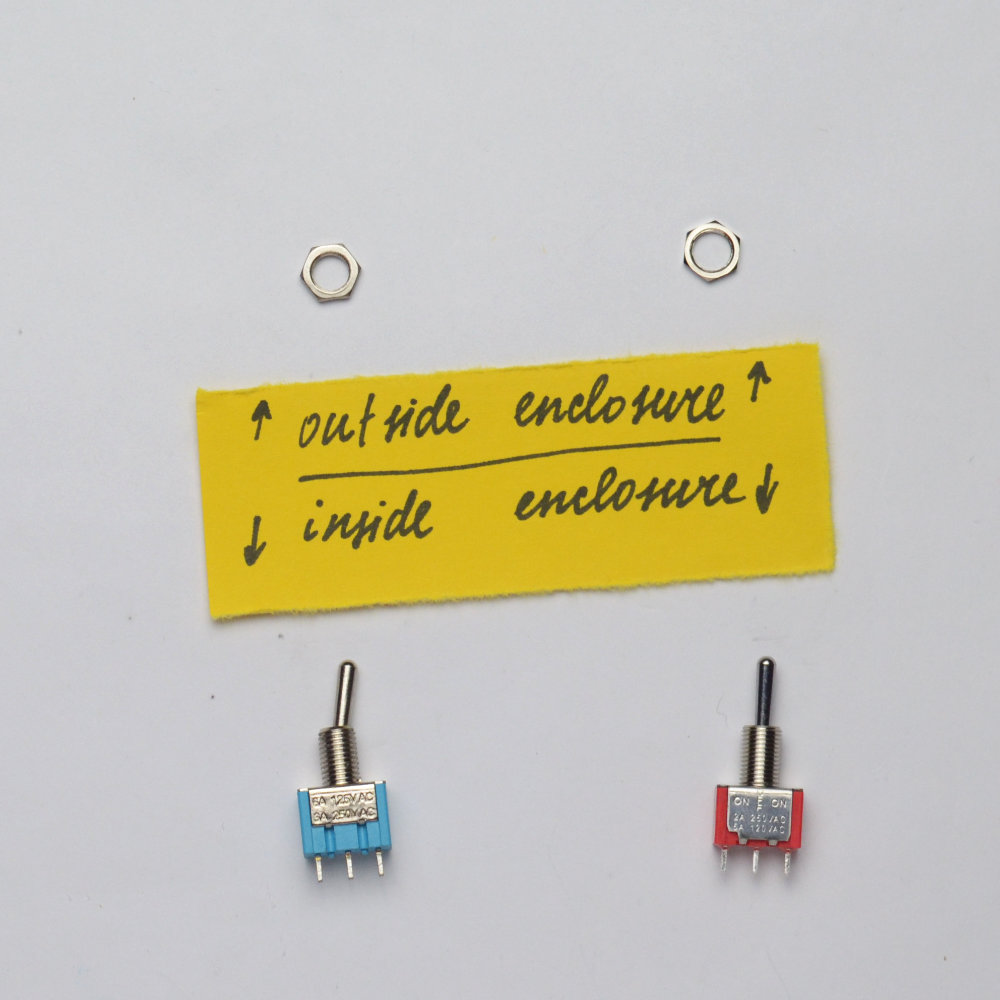
\includegraphics[width=\textwidth]{build/06-sw-mount-1000px.jpg}
  \end{subfigure}
  \begin{subfigure}[b]{0.49\textwidth}
    \centering
    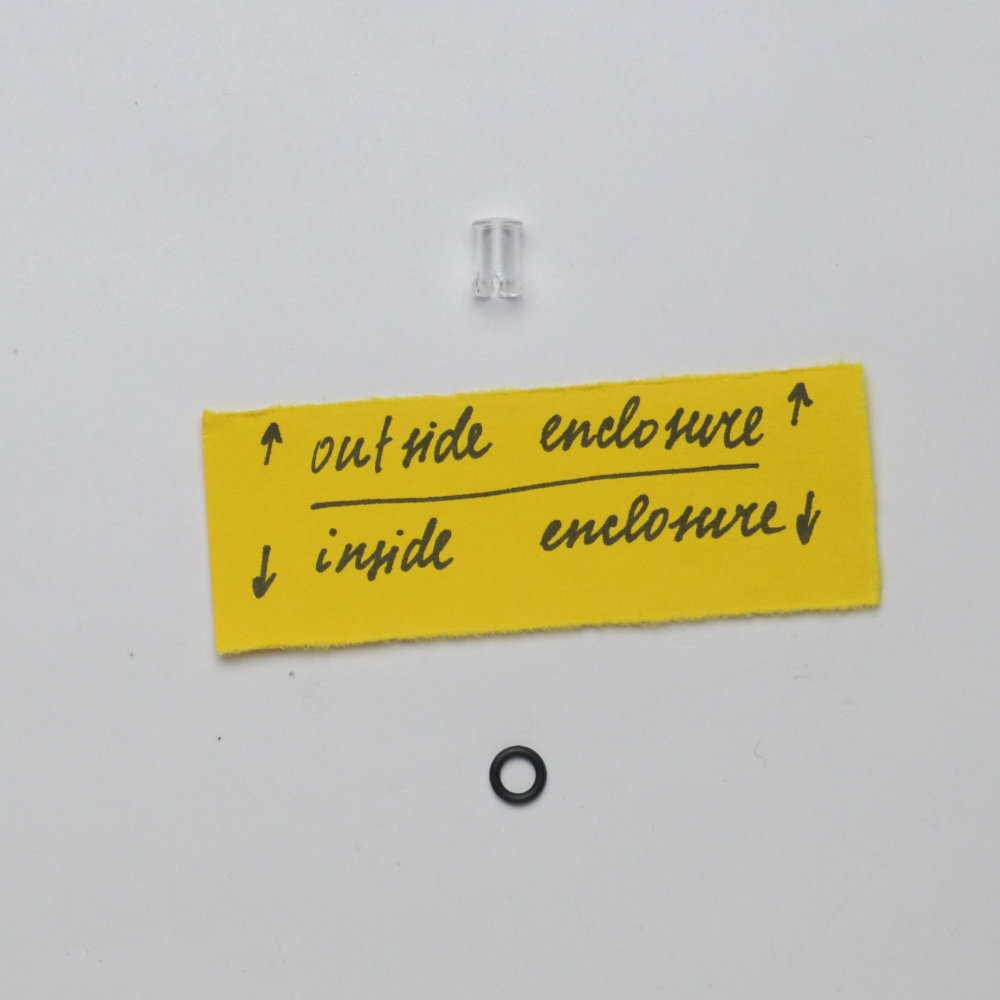
\includegraphics[width=\textwidth]{build/07-lampshade-mount-1000px.jpg}
  \end{subfigure}
  \caption{How to mount toggle switches and the lampshade}
\end{figure}

\restoregeometry{}

% \begin{figure}[h!]
%   \begin{center}
%     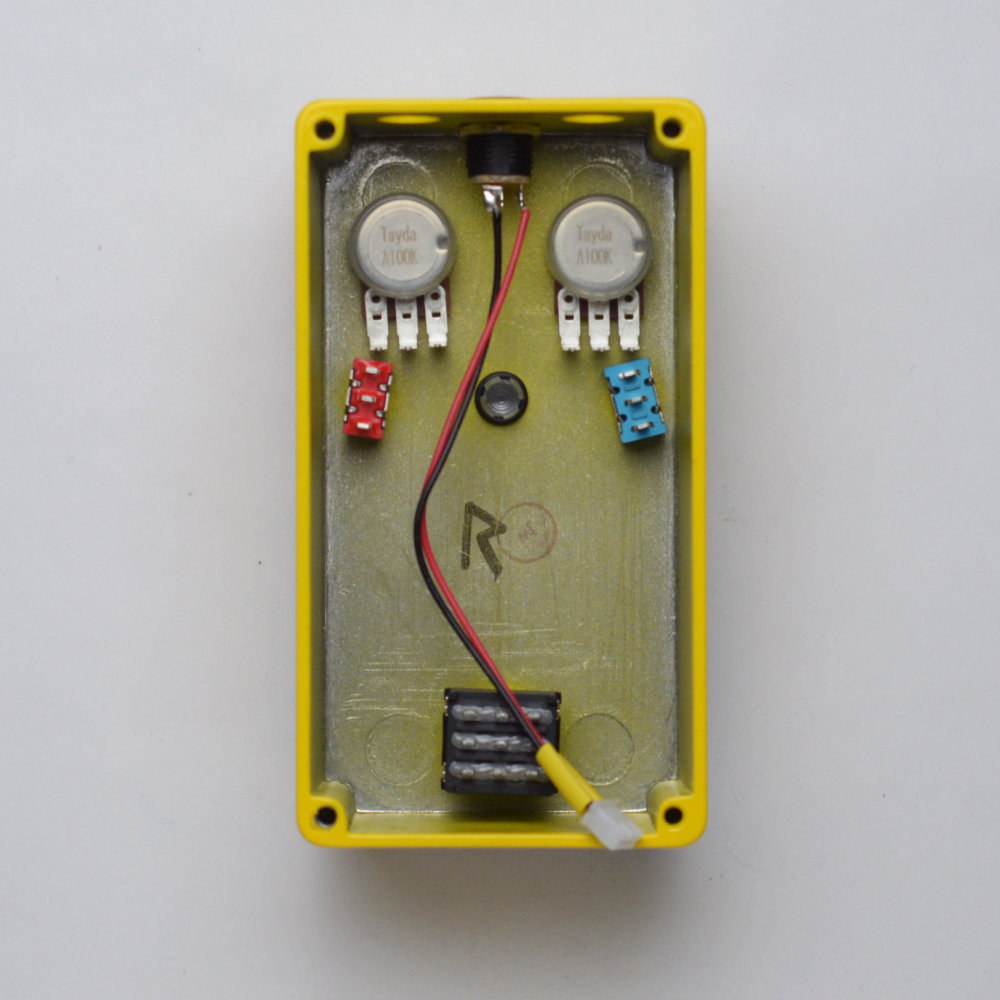
\includegraphics[width=0.7\textwidth]{build/09-enclosure-mount-inside-1000px.jpg}
%   \end{center}
%   \caption{Inside of the enclosure with parts mounted}
% \end{figure}


% \begin{figure}[h!]
%   \begin{center}
%     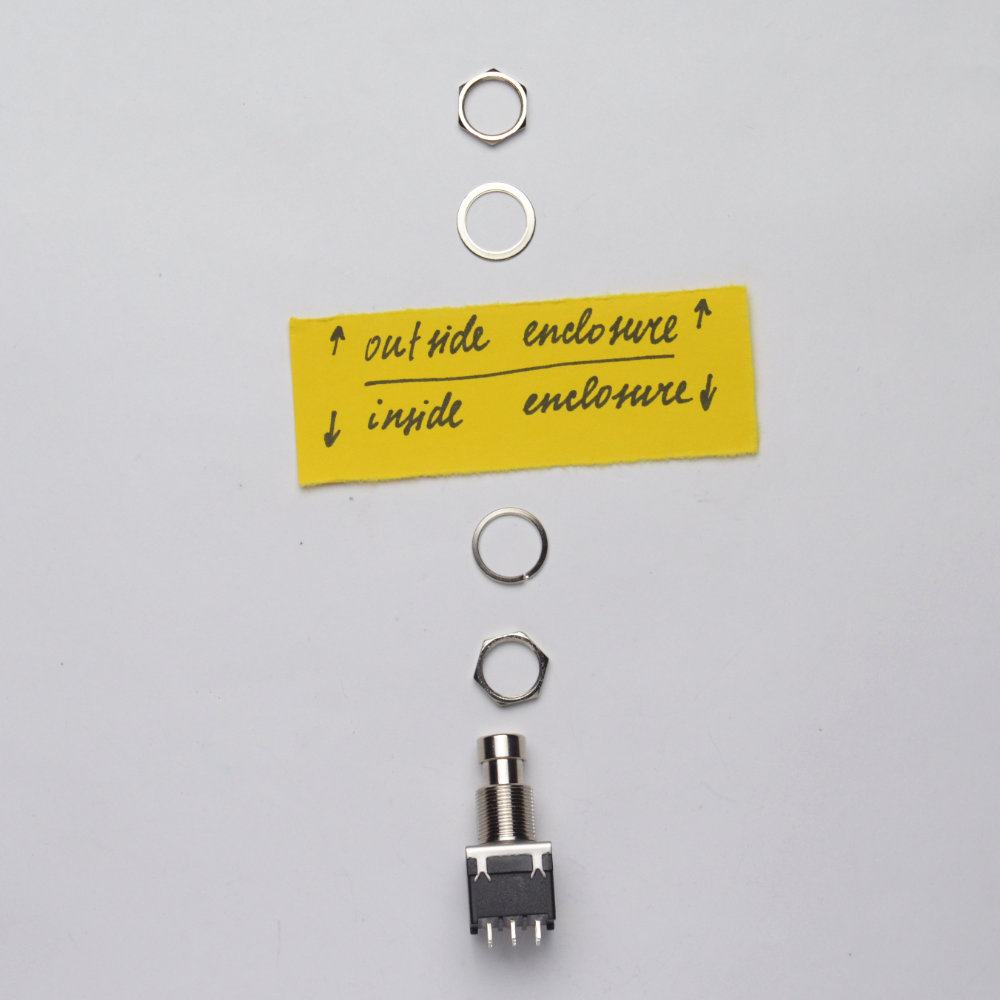
\includegraphics[width=0.5\textwidth]{build/05-fs-mount-1000px.jpg}
%   \end{center}
%   \caption{How to mount the footswitch}
% \end{figure}

% \begin{figure}[h!]
%   \begin{center}
%     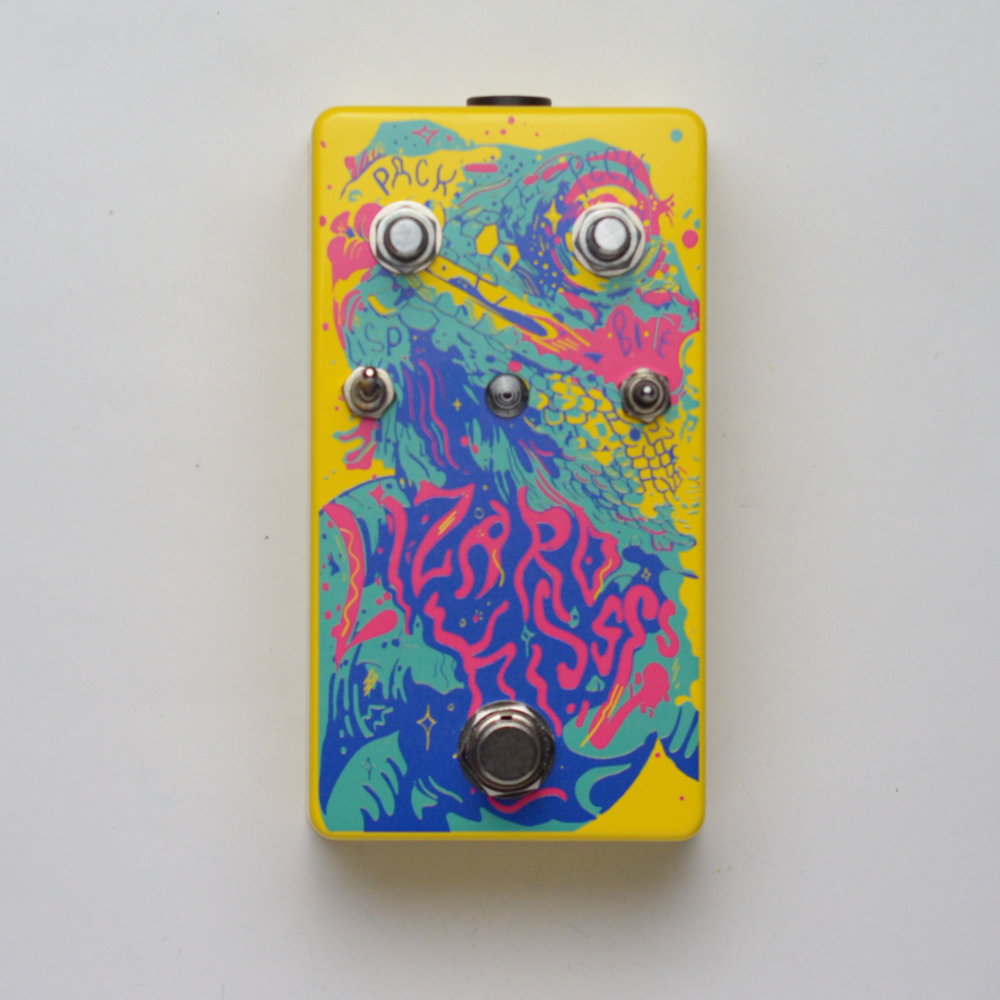
\includegraphics[width=0.7\textwidth]{build/08-enclosure-mount-1000px.jpg}
%   \end{center}
%   \caption{Outside of the enclosure with parts mounted}
% \end{figure}

\subsection{Populate main board}

\begin{itemize}
  \item Go through the \textbf{Main Board, floor side} section of the
    \hyperref[tbl:BOM]{BOM table} from top to bottom;
  \item One component at a time:
    \begin{itemize}
      \item Insert the part into the PCB;
      \item Flip the PCB and solder the part to the pads;
      \item Cut the excess component leads;
    \end{itemize}
\end{itemize}

\begin{figure}[h!]
  \centering
  \begin{subfigure}[b]{0.49\textwidth}
    \centering
    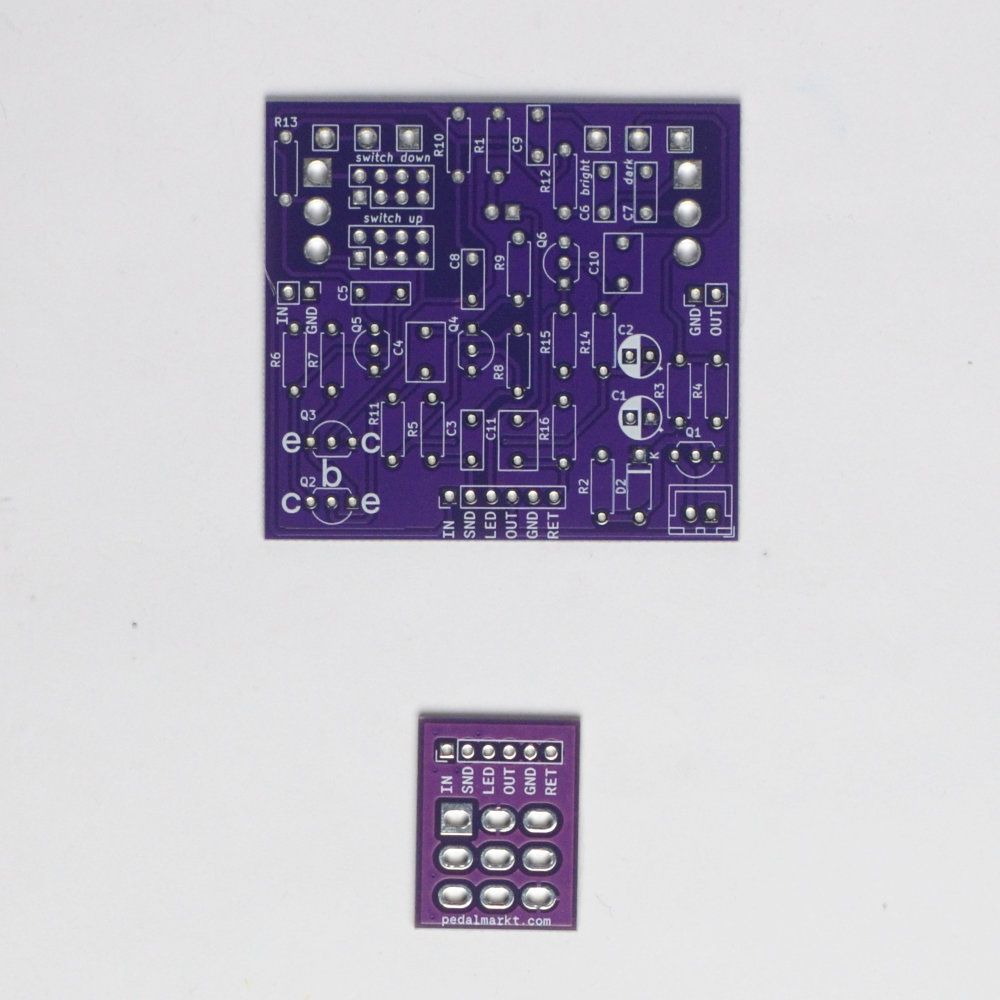
\includegraphics[width=\textwidth]{build/01-board-floor-1000px.jpg}
  \end{subfigure}
  \begin{subfigure}[b]{0.49\textwidth}
    \centering
    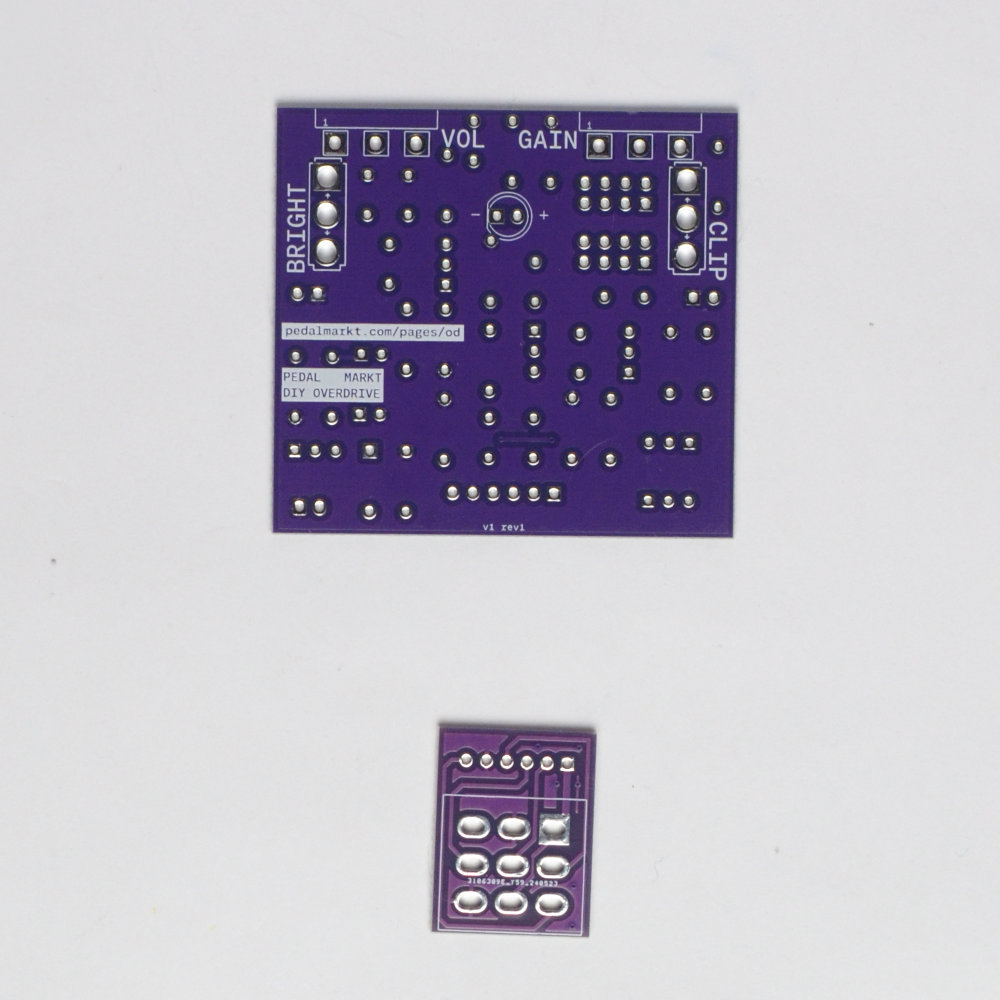
\includegraphics[width=\textwidth]{build/02-board-player-1000px.jpg}
  \end{subfigure}
  \caption{Main and switch boards, floor side on the left,
  player side on the right}
\end{figure}

\newgeometry{vmargin={3cm},hmargin={1cm}}

\begin{figure}[h!]
  \centering
  \begin{subfigure}[b]{0.49\textwidth}
    \centering
    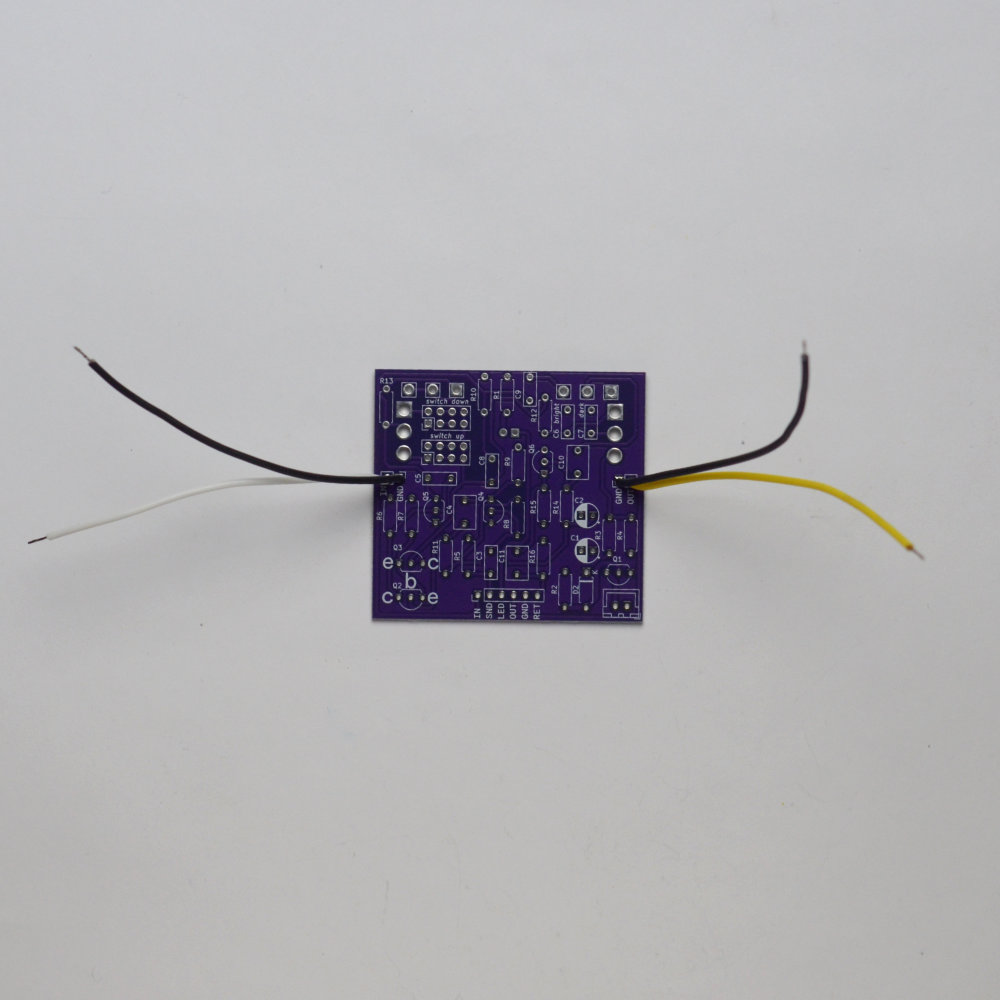
\includegraphics[width=\textwidth]{build/10-board-wires-1000px.jpg}
  \end{subfigure}
  \begin{subfigure}[b]{0.49\textwidth}
    \centering
    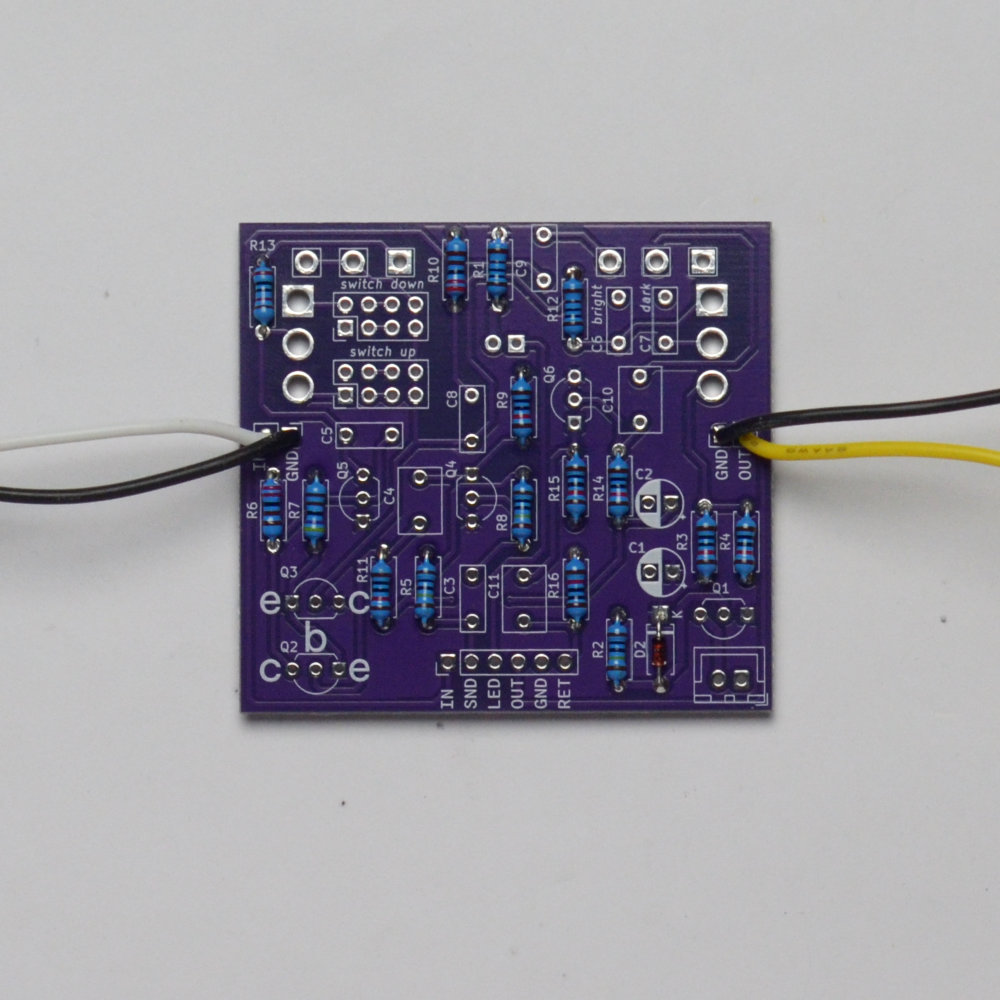
\includegraphics[width=\textwidth]{build/11-board-resistors-1000px.jpg}
  \end{subfigure}
  \caption{Wires soldered on the left, resistors on the right}
\end{figure}

\begin{figure}[h!]
  \centering
  \begin{subfigure}[b]{0.49\textwidth}
    \centering
    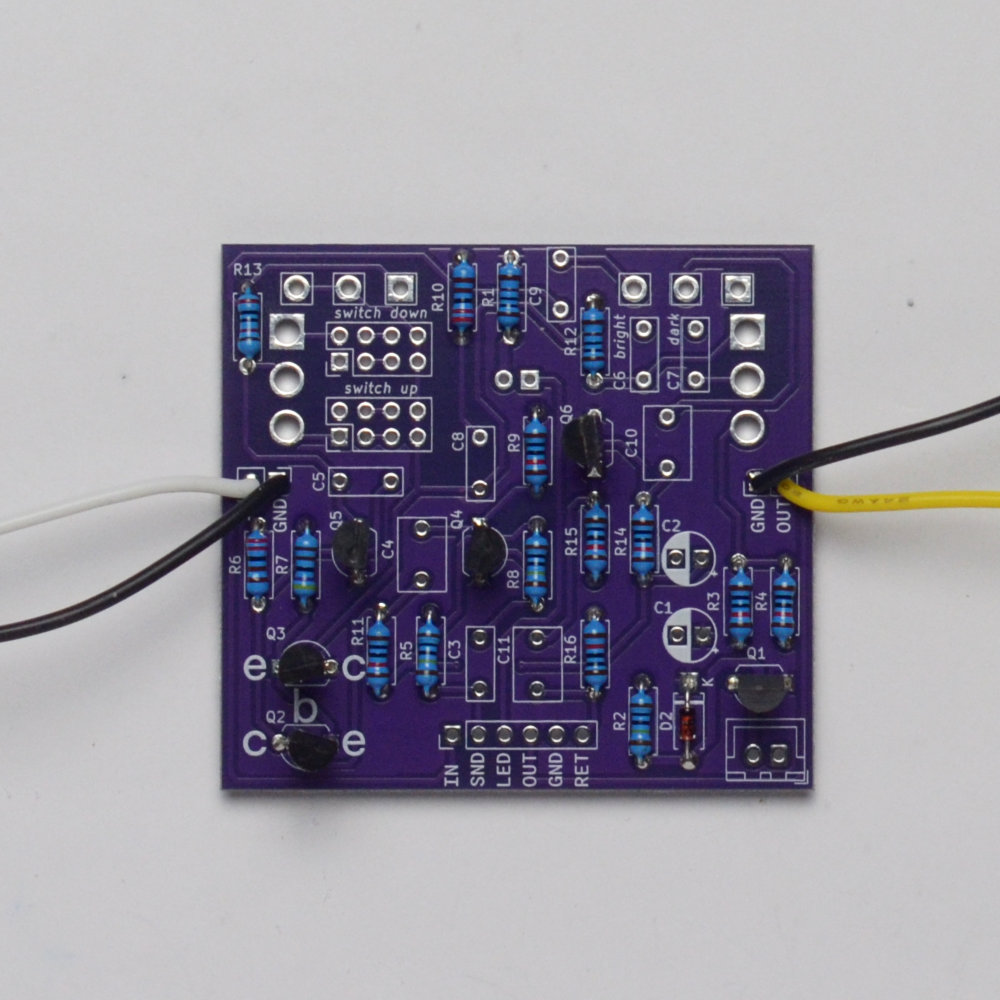
\includegraphics[width=\textwidth]{build/12-board-transistors-1000px.jpg}
  \end{subfigure}
  \begin{subfigure}[b]{0.49\textwidth}
    \centering
    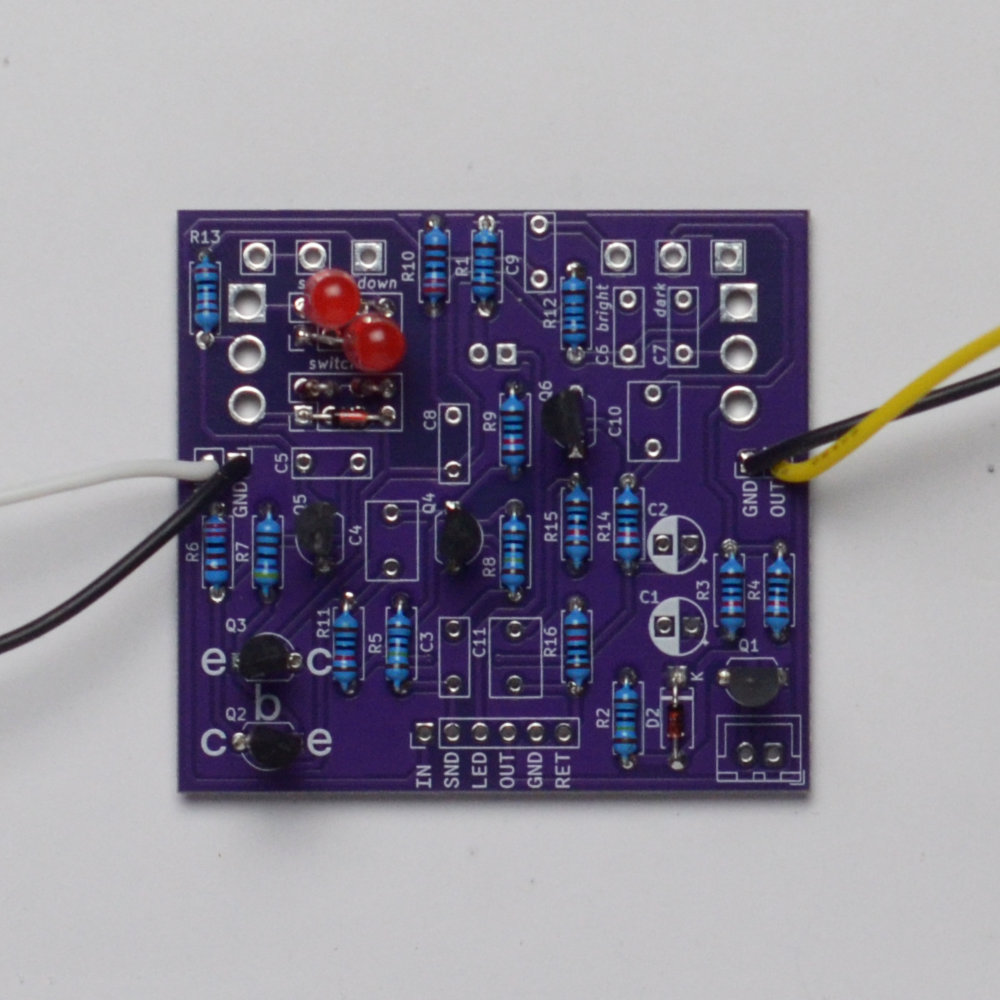
\includegraphics[width=\textwidth]{build/13-board-clipping-1000px.jpg}
  \end{subfigure}
  \caption{Transistors soldered on the left, diodes on the right}
\end{figure}

\begin{figure}[h!]
  \centering
  \begin{subfigure}[b]{0.49\textwidth}
    \centering
    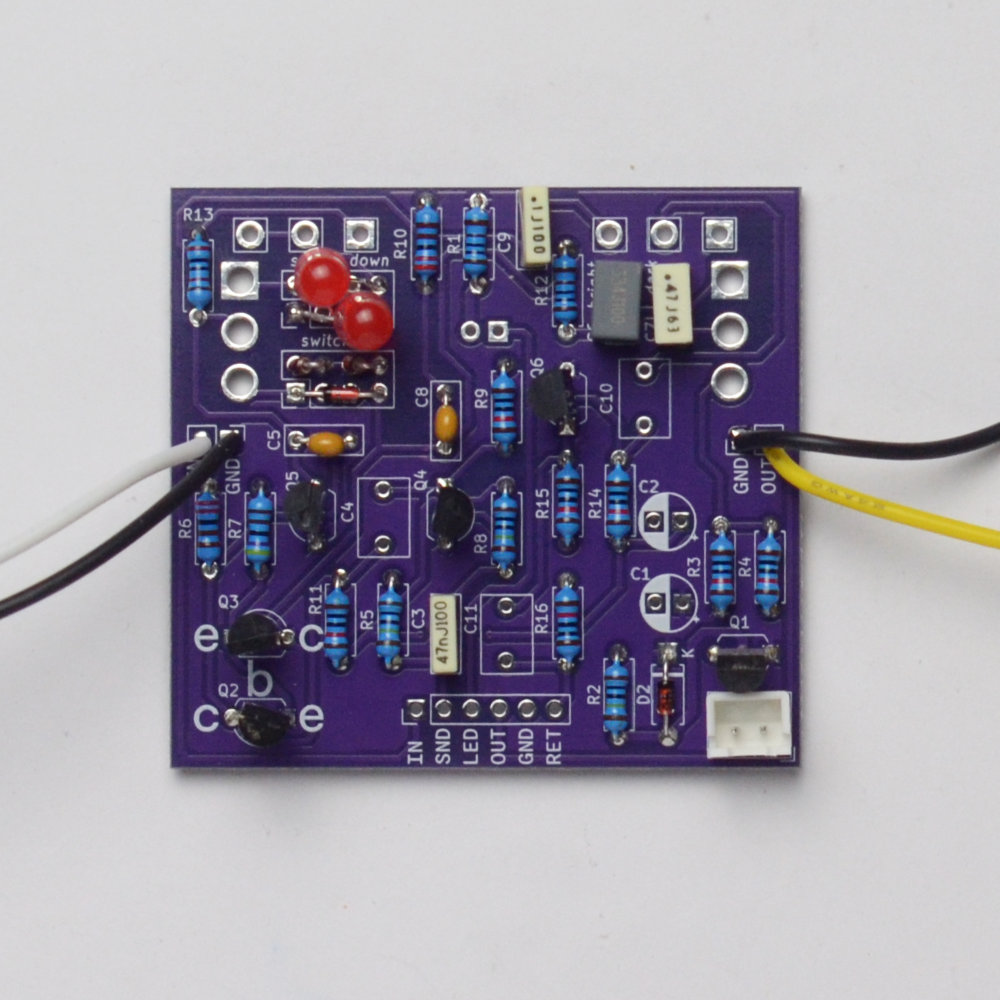
\includegraphics[width=\textwidth]{build/15-board-caps-1000px.jpg}
  \end{subfigure}
  \begin{subfigure}[b]{0.49\textwidth}
    \centering
    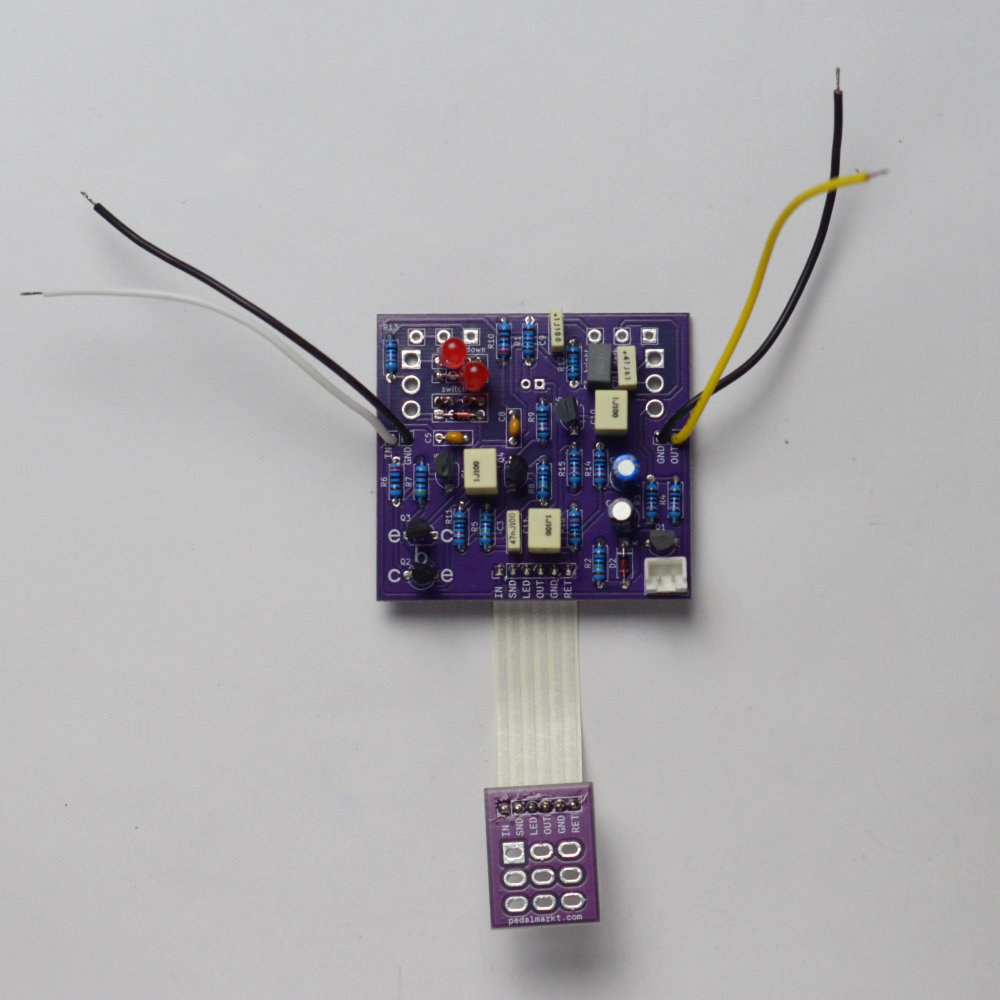
\includegraphics[width=\textwidth]{build/15-board-daughter-board-1000px.jpg}
  \end{subfigure}
  \caption{Caps soldered on the left, switch board and ribbon
  on the right}
\end{figure}


\restoregeometry{}

\subsection{Solder jacks and LED}

\begin{itemize}
  \item Solder audio jacks to the wires coming from the Main
    Board. Black (GND) wire should be connected to the lug
    that is connected to the round part on the inside of the
    jack socket. The colored wire (IN or OUT) should be
    connected to the other lug.
  \item Place the LED into the pads \textbf{on the player
    side} of the board. The short leg of the LED should go
    into the "-" (minus) pad. Do not solder the LED just
    yet.
\end{itemize}

\begin{figure}[h!]
  \centering
  \begin{subfigure}[b]{0.49\textwidth}
    \centering
    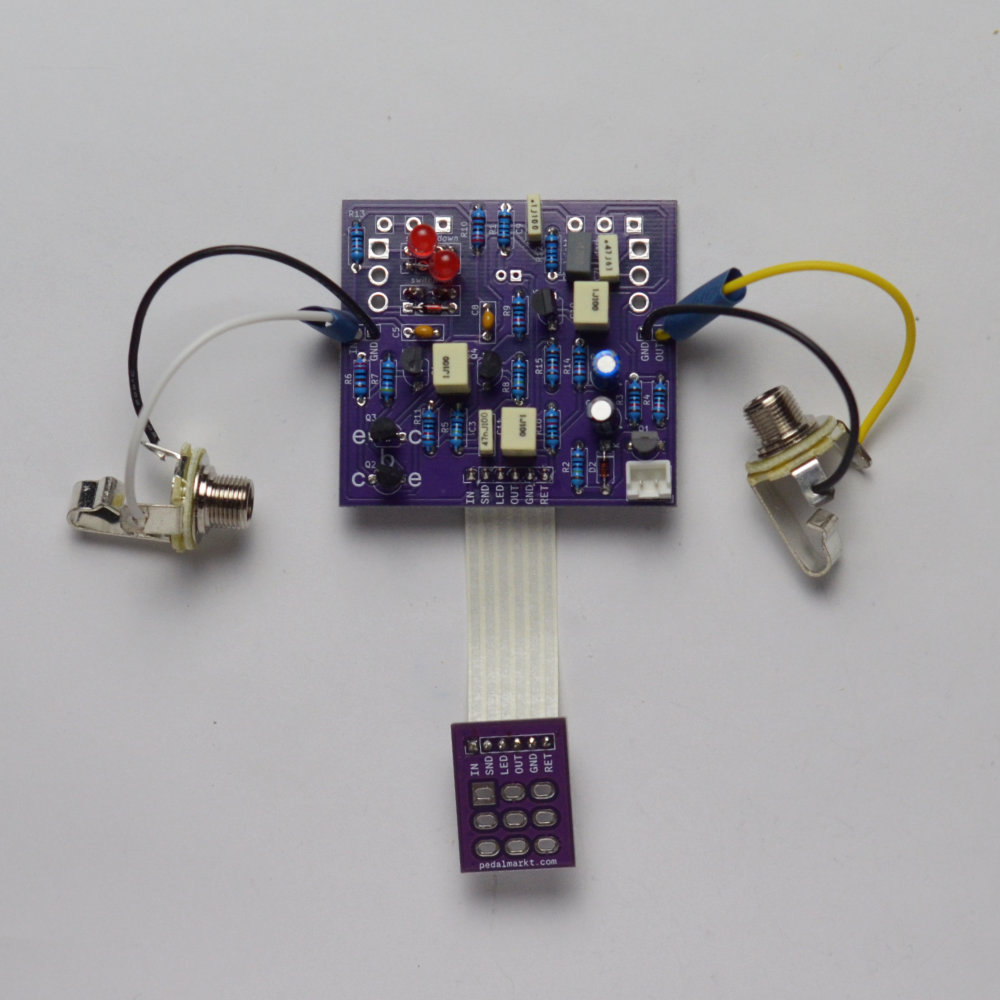
\includegraphics[width=\textwidth]{build/17-board-jacks-1000px.jpg}
  \end{subfigure}
  \begin{subfigure}[b]{0.49\textwidth}
    \centering
    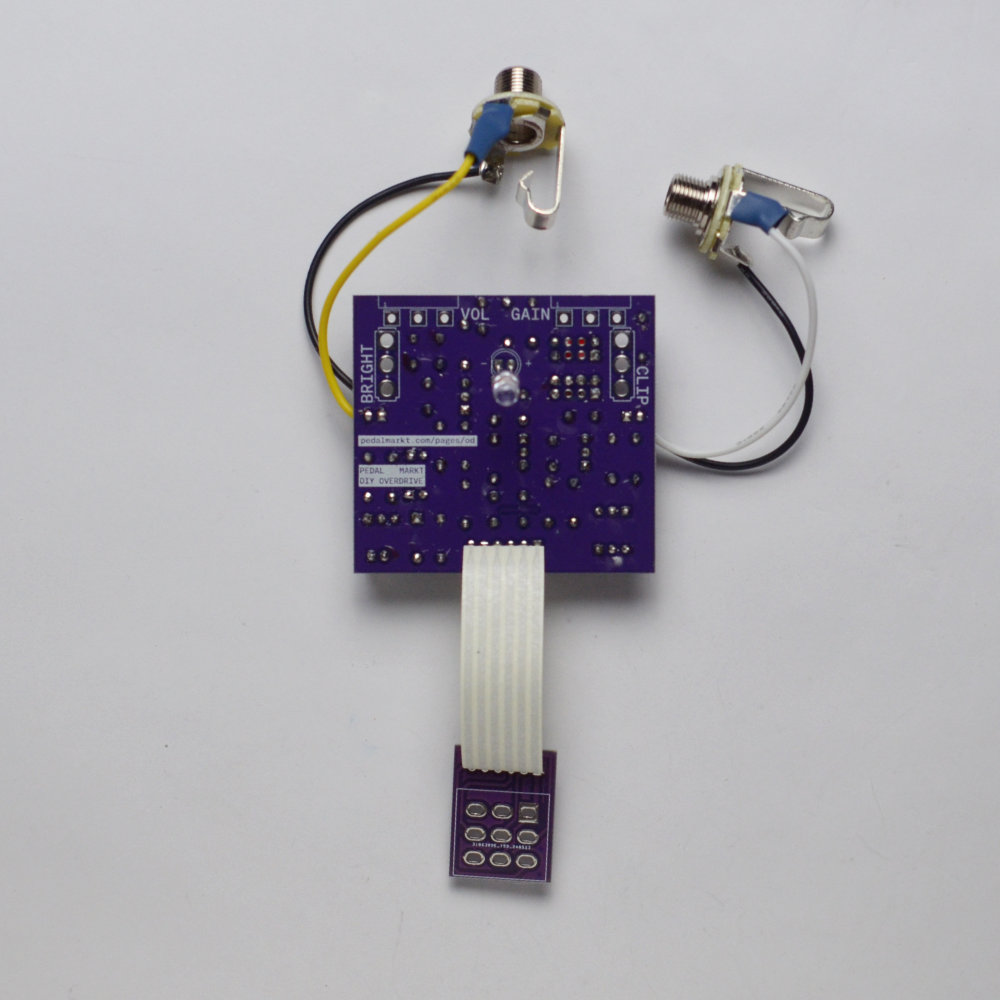
\includegraphics[width=\textwidth]{build/18-board-jacks-player-1000px.jpg}
  \end{subfigure}
  \caption{Audio jacks soldered on the left, LED placed but
  not soldered on the right}
\end{figure}

\pagebreak

\subsection{Mount boards into enclosure}

\begin{itemize}
  \item Place the main board into the enclosure, floor side
    of the board facing you;
    \begin{itemize}
      \item Make sure all the legs of the potentiometers and toggle
        switches get inserted into their dedicated pads;
      \item Make sure the LED gets inserted into the
        lampshade. You might have to press on the lampshade
        from the other side of the enclosure so that it
        doesn't lift from the enclosure;
      \item Solder the pots, the toggle switches and the LED to
        the main board;
    \end{itemize}
  \item Place the switch board onto the footswitch and
    solder them together.
\end{itemize}


\begin{figure}[h!]
  \begin{center}
    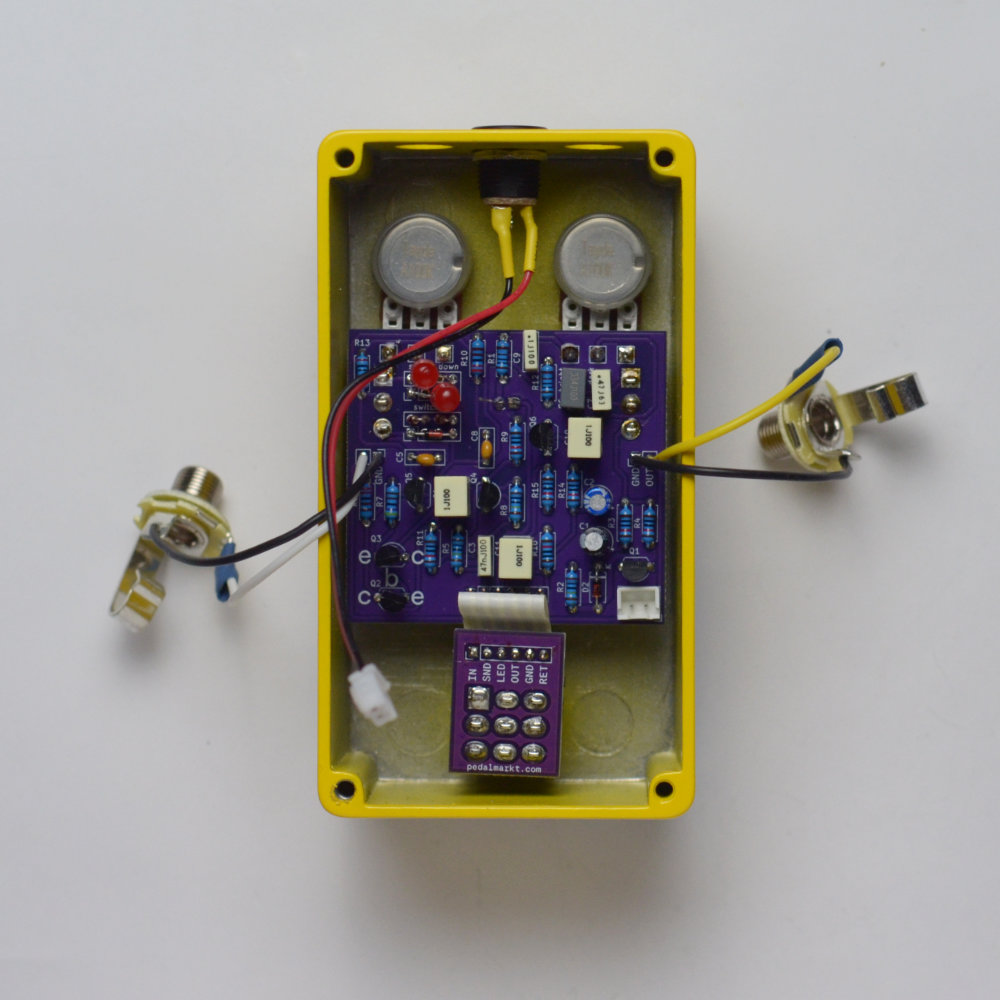
\includegraphics[width=0.8\textwidth]{build/19-board-enclosure-1000px.jpg}
  \end{center}
  \caption{Inside of the enclosure with boards mounted}
\end{figure}

\pagebreak

\subsection{Complete the pedal}

\begin{itemize}
  \item Mount the audio jacks onto the enclosure;
  \item Connect the DC cable to the socket on the bottom
    right of the board;
  \item Plug in and test the pedal!
\end{itemize}


\begin{figure}[h!]
  \begin{center}
    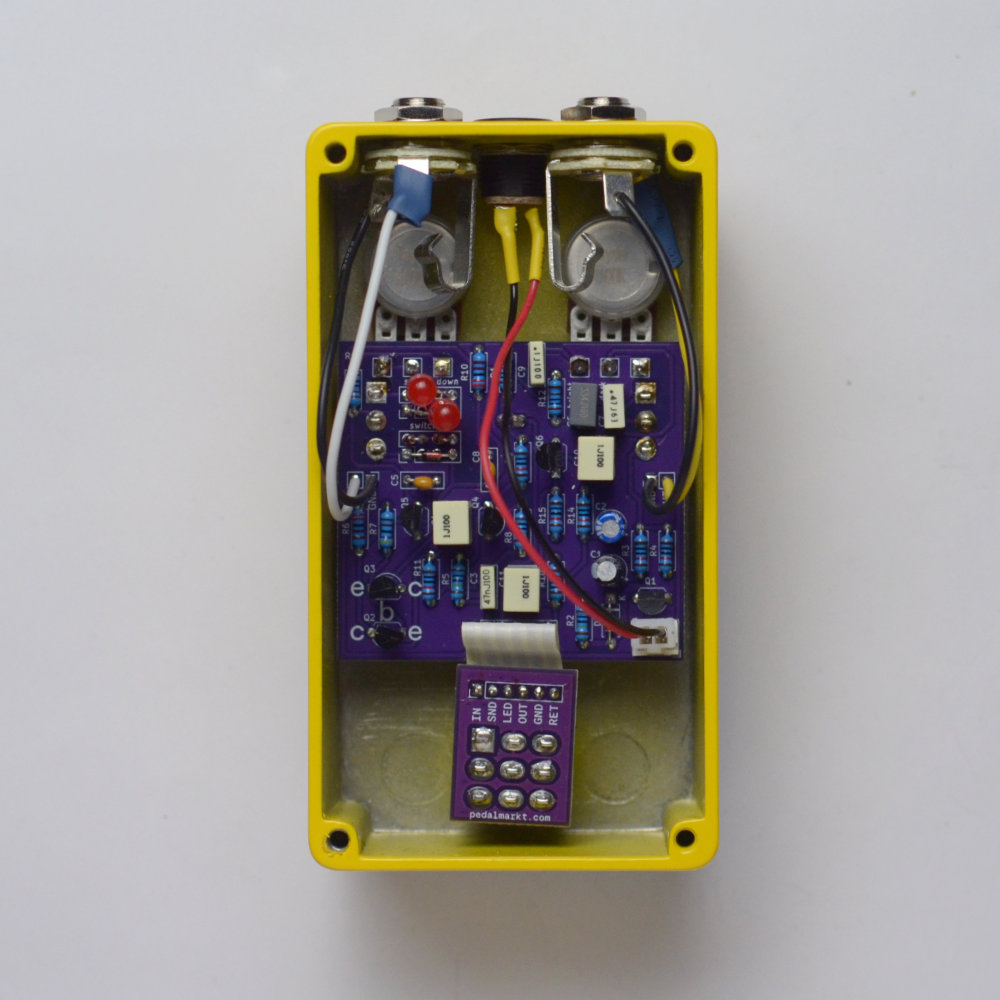
\includegraphics[width=\textwidth]{build/20-built-1000px.jpg}
  \end{center}
  \caption{Built pedal}
\end{figure}

\pagebreak

\section{Circuit breakdown}
\label{sec:circuit}

The core of the circuit is an amplifier, an active circuit
that makes an audio signal louder. We can wary the gain of
that amplifier. At some point, at higher gain settings the
signal 'wants' to get louder than what the circuit can
handle. It hits a ceiling and gets clipped. The more clipped
the signal is, the more distorted and compressed it sounds.

A specific kind of circuit that's used here is called a
non-inverting amplifier. Let's look at its basic version. The
gain here is proportional to the ratio of the two
resistors in its feedback loop: $R_{fb}/R_{gnd}$.

In our case, the Peck (Gain) control ($RV_1$ in schematic)
on the pedal varies $R_{fb}$.

\begin{figure}[h!]
\centering
\begin{circuitikz}[european]
\draw (3,0) node[above]{$v_i$} to[short, o-] ++(1,0)
node[op amp, anchor=+](OA){\texttt{Opamp}}
(OA.-) -- ++(-1,0) coordinate(FB)
to[R=$R_{gnd}$] ++(-2,0) node[ground]{}
(FB) to[short, *-] ++(0,1) coordinate(FBTop) to[R=$R_{fb}$] (FBTop -| OA.out) -- (OA.out)
to [short, *-o] ++(1,0) node[above]{$v_o$}
;
\end{circuitikz}
\caption{Non-inverting amplifier based on an opamp}
\end{figure}

There are a few  changes to that basic circuit. First, there
is a capacitor in the feedback loop of the opamp. Its role
is to affect which frequencies get amplified. In other
words, $C_{gnd}$ in combination with $R_{gnd}$ acts as a
high-pass filter.

The value of the capacitor $C_{gnd}$ is what the LISP
(Brightness) toggle is switching ($C_6$ or $C_6+C_7$ in
schematic).

\begin{figure}[h!]
\centering
\begin{circuitikz}[european]
\draw (5,0) node[above]{$v_i$} to[short, o-] ++(1,0)
node[op amp, anchor=+](OA){\texttt{Opamp}}
(OA.-) -- ++(-1,0) coordinate(FB)
(FB) to[R=$R_{gnd}$] ++(-2,0) to[C=$C_{gnd}$] ++(-1,0) node[ground]{}
(FB) to[short, *-] ++(0,1) coordinate(FBTop) to[R=$R_{fb}$] (FBTop -| OA.out) -- (OA.out)
to [short, *-o] ++(1,0) node[above]{$v_o$}
;
\end{circuitikz}
\caption{Non-inverting amplifier with a high-pass filter}
\end{figure}

To make the distortion effect  more intense we can put
clipping diodes into the feedback loop of the opamp, see
\nameref{fig:oadi}.

\begin{figure}[h!]
\centering
\begin{circuitikz}[european]
\draw (5,0) node[above]{$v_i$} to[short, o-] ++(1,0)
node[op amp, anchor=+](OA){\texttt{Opamp}}
(OA.-) -- ++(-1,0) coordinate(FB)
(FB) to[R=$R_{gnd}$] ++(-2,0) to[C=$C_{gnd}$] ++(-1,0) node[ground]{}
(FB) to[short, *-] ++(0,1) coordinate(FBTop) to[R=$R_{fb}$] (FBTop -| OA.out) -- (OA.out)
(FBTop) to[short, *-] ++(0,1.5) coordinate(FBD1) to[D=$D_1$] (FBD1 -| OA.out) -- (FBTop -| OA.out) to[short, *-] +(0,0)
(FBD1) to[short, *-] ++(0,1.5) coordinate(FBD2) to[D=$D_2$,invert] (FBD2 -| OA.out) -- (FBD1 -| OA.out) to[short, *-] +(0,0)
(OA.out) to [short, *-o] ++(1,0) node[above]{$v_o$}
;
\end{circuitikz}
\caption{\label{fig:oadi}Non-inverting amplifier with a high-pass filter and
  clipping diodes}
\end{figure}


Another important note about the way Lizard Kisses
implements the non-inverting amplifier is it's using a
discrete opamp. Discrete means it's built out of single
transistors, as opposed to an integrated circuit aka a chip.
$DOA_+$, $DOA_-$ and $DOA_{out}$ in the schematic correspond
to the positive, negative, and output terminals on the
abstract opamp above.

The rest of the circuit is pretty standard:

\begin{itemize}
  \item Transistor $Q_4$ and surrounding components form an
    input buffer;
  \item Transistor $Q_6$ and surrounding components form an
    output buffer;
  \item Pot $RV_2$ is a volume control used to compensate
    for the added gain;
  \item MOSFET $Q_1$ and surrounding components form a
    reverse voltage protection circuit;
\end{itemize}

\pagebreak

\section{Schematic}
\label{sec:schematic}

\begin{figure}[h!]
  \centering
  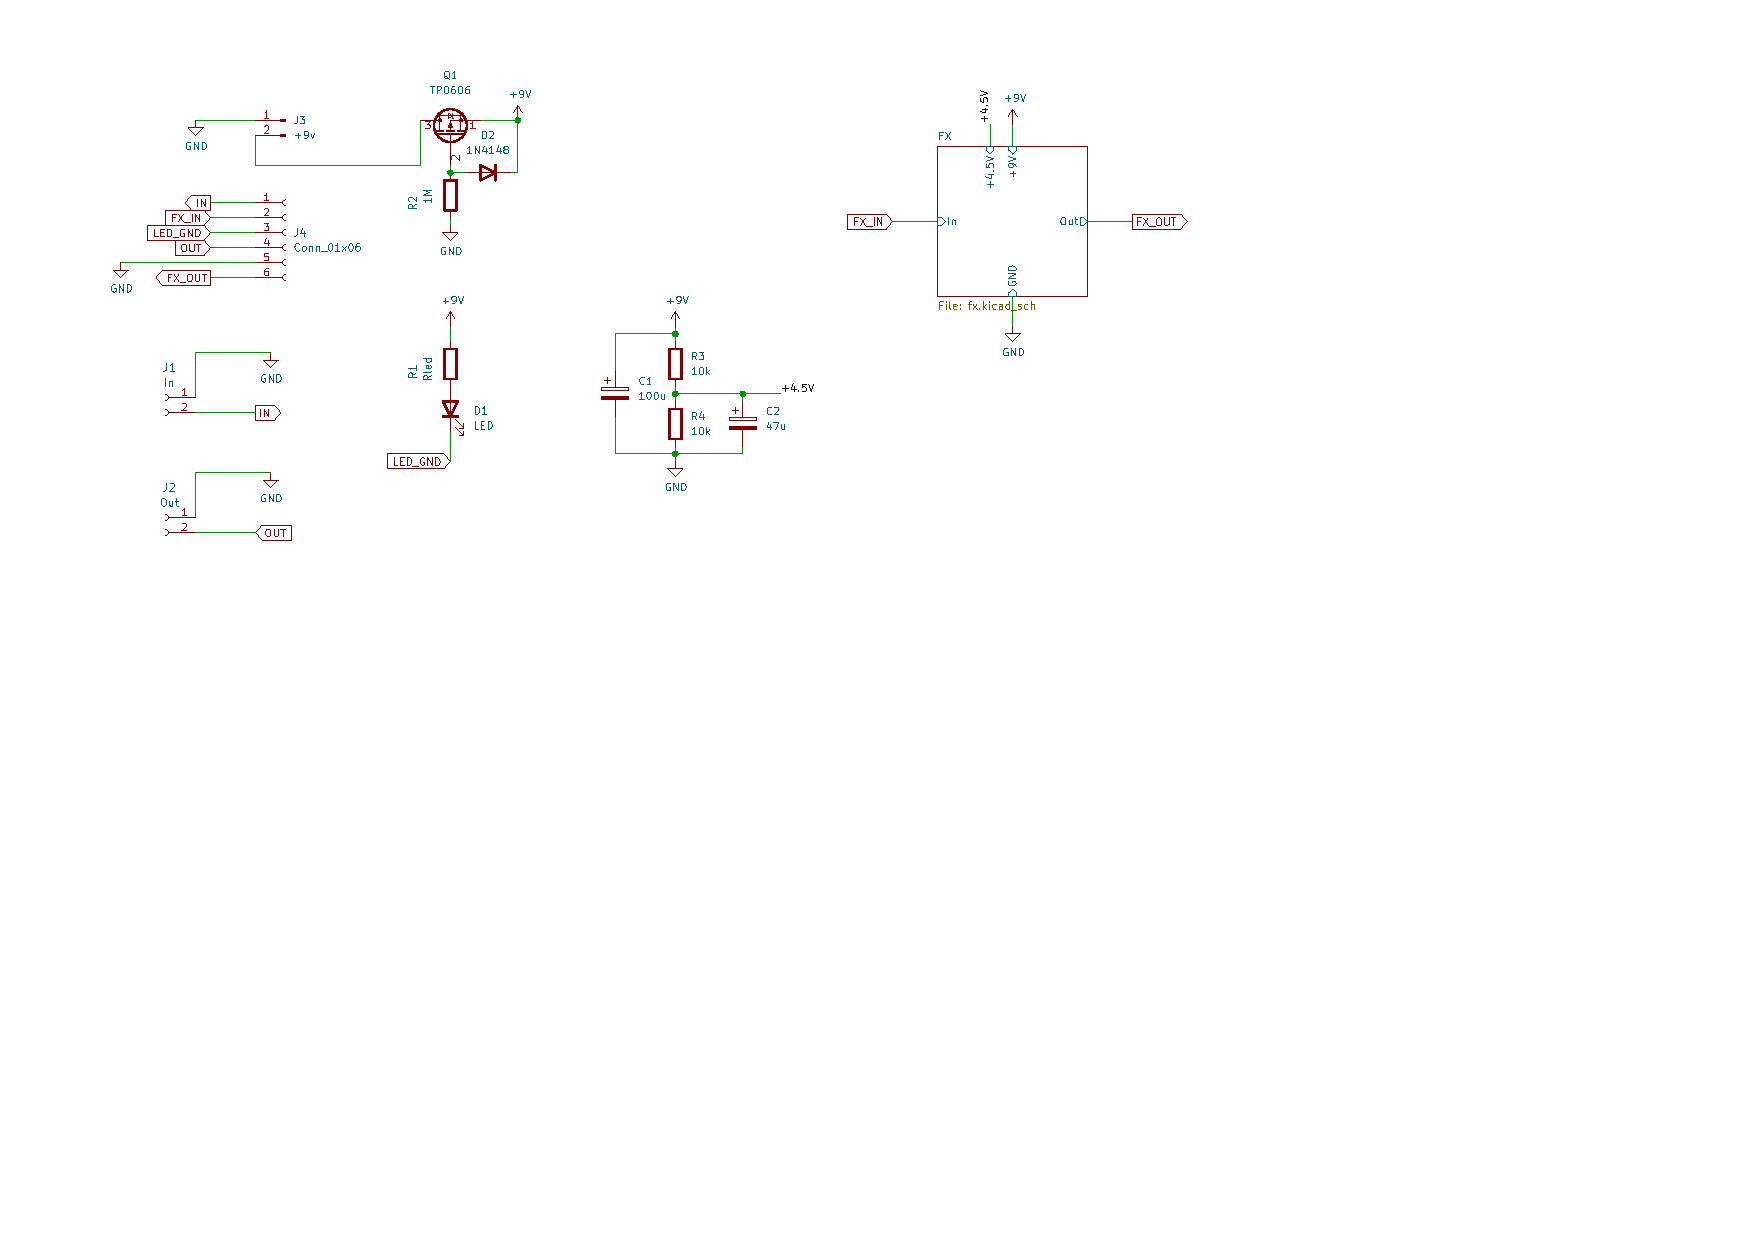
\includegraphics[width=1.3\textwidth, trim={0 10cm 6cm 0cm}, clip, angle=-90]{schem.pdf}
\end{figure}

\begin{figure}[h!]
  \centering
  \includegraphics[width=1.3\textwidth, trim={0 4cm 0cm 0cm}, page=2, clip, angle=-90]{schem.pdf}
\end{figure}


\end{document}
